%RATRAPER COURS 1 
\chapter{Some basics of statistical learning}

\underline{Nouveau cours du 15/11} 

$\mathcal{D}_n = {(X_1, Y_1), \dots, (X_n,Y_n)}$ training samples iid copies of $(X,Y)$. $X \in \mathcal{X}$ and $Y \in \mathcal{Y}$ 

\begin{itemize}
    \item \textbf{goal} : fing a predictor surch that $f(X_i) \simeq Y_i$ on the training set. \\
    but above all $f(X_{\text{new}}) \simeq Y_{\text{new}}$ (test set) 
    \item \textbf{Risk} : $\mathcal{R}^{\textcolor{green}{(l)} }(f) = \underarrow[\mathbb{E}][\uparrow]{\textcolor{red}{on (X,Y)}} [ \overarrow[\ell][\downarrow]{\textcolor{green}{loss}}(Y, f(X))]$
    \item \textbf{Bayes predictor} : $f^\ast  \in \arg \min \mathcal{R}(f)$ \\
    $ \mathcal{R}^\ast = \mathcal{R}(f^\ast) = \inf \limits_{f} \mathcal{R}(f) $
    \item \textbf{Empirical risk} : $\hat{\mathcal{R}}_n (f) := \frac{1}{n} \sum \limits_{i=1}^{n} \ell (Y_i, f(X_i))$ \\
    $\hat{f}^{\text{ERM}} \in  \arg \min \limits_f \hat{\mathcal{R}}_n (f) $ (On some class of predictor)
\end{itemize}

Statistical learning theory focuses on controlling 
\[
    \mathcal{R}_n (\hat{f}_n) - \mathcal{R}^\ast  \text{  or  } \hat{\mathcal{R}}_n (\hat{f}_n) - \mathcal{R}^\ast
\]
for $\hat{f}_n$ a constructed predictor on the training set of size $n$. \\

\textbf{Classical error decomposition} :
\[
    \mathcal{R} (\hat{f}_n) - \mathcal{R}^\ast = 
    \textcolor{violet}{\underbrace{\color{black}\inf_{f \in \mathcal{F}} \mathcal{R}(f) - \mathcal{R}^\ast }_{\text{approximation error}} } 
    + \textcolor{cyan}{\underbrace{\color{black} \mathcal{R}(\hat{f}^\text{ERM}) - \inf_{f \in \mathcal{F}} \mathcal{R}(f) }_{\text{estimation error}} }
    +  \textcolor{gray}{\underbrace{\color{black} \mathcal{R} (\hat{f}_n) - \mathcal{R}(\hat{f}^\text{ERM}) }_{\substack{\text{error due to the use of an} \\ \text{ optimisation algo for ERM} } }}
.\]


%\begin{wrapfigure}{r}{0.4\textwidth}
%    \centering
%    \vfill
%    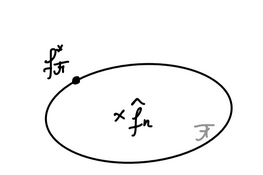
\includegraphics[width=0.35\textwidth]{figs/overfitting_ERM.png}
%    \caption{Overfitting for ERM}
%    \vfill  
%\end{wrapfigure} 

\begin{figure}[h]
    \begin{minipage}{0.5\textwidth}
        \textbf{Control of the estimation error} \\
        "Overfitting" : we have 
        \[
            \textcolor{gray}{\underbrace{\color{black} \hat{\mathcal{R}}_n (\hat{f}_n) }_{\text{train risk}  }}
            <<<
            \textcolor{gray}{\underbrace{\color{black} \mathcal{R}_n (\hat{f}_n) }_{\text{test risk}  }}
        .\]
    \end{minipage}
    \begin{minipage}{0.5\textwidth}
        \centering
        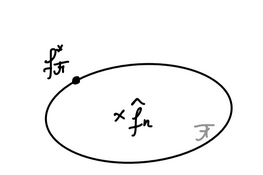
\includegraphics[width=0.8\textwidth]{figs/overfitting_ERM.png}
        \caption{Overfitting for ERM.}
        %\label{fig:figure}
    \end{minipage}
\end{figure}


\begin{lem}[]
    For the ERM predictor $\hat{f}_n = \hat{f}^{\text{ERM}}$, one has 
    \[
        \mathcal{R}(\hat{f}^{\text{ERM}}) - \mathcal{R}(f^\ast _{\mathcal{F}}) \leq 2 \sup_{f \in \mathcal{F}} \left| \hat{\mathcal{R}_n} - \mathcal{R} \right| (f)
    .\]
    with $f^\ast _{\mathcal{F}} \in \arg \min \limits_{f \in \mathcal{F}}\mathcal{R}(f)$
\end{lem}

Meaning the there is a link between estimation error and control of empirical process.

\begin{proof}[Preuve : ]
    \begin{align*}
        \mathcal{R} (\hat{f}^{\text{ERM}}) - \mathcal{R}(f^\ast _{\mathcal{F}}) 
        & = \textcolor{gray}{\underbrace{\color{black} \mathcal{R} (\hat{f}^{\text{ERM}}) \textcolor{blue}{-} \hat{\mathcal{R}}_n(\hat{f}^{\text{ERM}})}_{\leq \sup\limits_{f \in \mathcal{F}} ( \hat{\mathcal{R}_n} - \mathcal{R} ) (f) } }
        \textcolor{blue}{+} \textcolor{gray}{\underbrace{ \color{black} \hat{\mathcal{R}}_n(\hat{f}^{\text{ERM}}) \textcolor{red}{-} \hat{\mathcal{R}}_n(f^\ast_ \mathcal{F} ) }_{\leq 0 \text{ by optimality of } \hat{f}^{\text{ERM}} }}
        \textcolor{red}{+} \textcolor{gray}{\underbrace{ \color{black} \hat{\mathcal{R}}_n(f^\ast_ \mathcal{F} ) - \mathcal{R}(f^\ast _{\mathcal{F}}) }_{\leq \sup\limits_{f \in \mathcal{F}} ( \hat{\mathcal{R}_n} - \mathcal{R} ) (f) }} \\
        &\leq 2 \sup_{f \in \mathcal{F}} \left| \hat{\mathcal{R}_n} - \mathcal{R} \right| (f)
    \end{align*}
\end{proof}


Technics to control the supremum of empirical process.
\begin{itemize}
    \item In expectation : $\mathbb{E}[ \mathcal{R}(\hat{f}^\text{ERM}) - \mathcal{R}(f^\ast _{\mathcal{F}})]$ small? \\
    tool : Pisier's lemma
    \item in proba : $\mathbb{P}(\mathcal{R}(\hat{f}^\text{ERM}) - \mathcal{R}(f^\ast _{\mathcal{F}}) > \varepsilon ) \leq \delta $ \\
    tool : union bound + Hoeffding inequality
\end{itemize}

\begin{thm}[Hoeffding's inequality]
    $X_1, \dots X_n \ind$ r.v. and $X_i \in [a_i, b_i]$ a.s. \\
    then \begin{align*}
        \mathbb{P}(\left| \frac{1}{n} \sum_{i=1}^{n} (X_i - \mathbb{E}[X_i]) \right| > \varepsilon ) 
        & \leq 2 e^{-\dfrac{2 n ^2 \varepsilon ^2}{\sum_{i}^{} (b_i - a_i)^2}} \\
        \text{when} \begin{cases}
             &a_i =a\\
             &b_i =b\\
        \end{cases} \quad \rightarrow  & \leq  2 e^{-\dfrac{2 n \varepsilon ^2}{(b - a)^2}}
    \end{align*} 
\end{thm}

\begin{enumerate}
    \item When $n to + \infty $ ($\varepsilon $ fixed) the bound goes to 0.
    \item When $b -a \to + \infty $ the bound goes to 1.
    \item The R.H.S (right hand side) should depend on $\frac{\varepsilon }{b-a}$ (One could rescale $X_i$ by $\frac{1}{b-a}$ )
    \item By the CLT, the R.H.S should go to a constant if $n \to \infty $ and $\varepsilon = \frac{\tau }{\sqrt[]{n}}$ \begin{align*}
        \mathbb{P} ( \frac{1}{n} \sum_{i=1}^{n} (X_i &- \mathbb{E}[X_i]) >  \frac{\tau }{\sqrt[]{n}}) =  \mathbb{P}( \frac{1}{\sqrt{n}} \sum_{i=1}^{n} (X_i - \mathbb{E}[X_i]) >  \tau) \\
        & \xrightarrow[n \to \infty]{} \mathbb{P}(\mathcal{N}(0, . ) > \tau ) = \text{ constant }(\tau )
    \end{align*}
\end{enumerate}

\begin{prop}[]
    In the case of binary classification ($y = \{+1, -1\}$), concider a finite class $\mathcal{F}$ of predictors, i.e. of cardinality $\left| \mathcal{F} \right| < + \infty $. 
    \[
        \mathbb{P}(\sup _{f \in  \mathcal{F}} \left| \hat{\mathcal{R}}_n - \mathcal{R} \right|(f)> \varepsilon  ) \leq 2 \left| \mathcal{F} \right| e^{-2n \varepsilon^2} 
    .\]
\end{prop}

\begin{proof}[Preuve : ]
    \begin{align*}
        \mathbb{P}(\sup_{f in \mathcal{F}} \left| \hat{\mathcal{R}}_n - \mathcal{R} \right| (f) > \varepsilon  ) 
        &= \mathbb{P} ( \bigcup _{f \in \mathcal{F}} \{ \left| \hat{\mathcal{R}}_n - \mathcal{R} \right| (f) > \varepsilon \}) \\
        & \leq \sum_{f in \mathcal{F}}^{} \mathbb{P}(\left| \hat{\mathcal{R}}_n - \mathcal{R} \right| (f) > \varepsilon ) \qquad \text{[Union bound]}
    \end{align*}

    But $\left| \hat{\mathcal{R}}_n - \mathcal{R} \right| (f) = \frac{1}{n} \left| \sum_{i=1}^{n} \mathbbm{1}_{f(X_i) \neq Y_i} - \mathbb{E}[\mathbbm{1}_{f(X_i) \neq Y_i}] \right| = \frac{1}{n} \left| \sum_{i=1}^{n} Z_i - \mathbb{E}[Z_i] \right| $ \\
    with $Z_i \in \{0, 1\} \in [0,1]$ \\
    Therefore $\forall f \in  \mathcal{F}, \mathbb{P}(\left| \hat{\mathcal{R}}_n - \mathcal{R} \right| (f) > \varepsilon ) \leq 2 e^{-2n \varepsilon ^2}$. \\
    Finally, $$\mathbb{P}(\sup _{f \in  \mathcal{F}} \left| \hat{\mathcal{R}}_n - \mathcal{R} \right|(f)> \varepsilon  ) \leq 2 \left| \mathcal{F} \right| e^{-2n \varepsilon^2} $$
\end{proof}


\textcolor{red}{TO BE COMPLETED}
